
%----------------------------------------------------------------------------------------
%    PACKAGES AND OTHER DOCUMENT CONFIGURATIONS
%----------------------------------------------------------------------------------------

\documentclass{article}

\usepackage{fancyhdr} % Required for custom headers
\usepackage{lastpage} % Required to determine the last page for the footer
\usepackage{extramarks} % Required for headers and footers
\usepackage{graphicx} % Required to insert images
\usepackage{mathtools, bm}
\usepackage{amssymb, bm}
\usepackage{graphicx}
\usepackage{float}
\usepackage{multirow}
\usepackage[table]{xcolor}  
\usepackage{algorithm}
\usepackage[noend]{algpseudocode}

% Margins
\topmargin=-0.45in
\evensidemargin=0in
\oddsidemargin=0in
\textwidth=6.5in
\textheight=9.0in
\headsep=0.25in


\linespread{1.1} % Line spacing

% Set up the header and footer
\pagestyle{fancy}
\lhead{\hmwkAuthorName} % Top left header
\chead{\hmwkTitleComp} % Top center header
\rhead{\firstxmark} % Top right header
\lfoot{\lastxmark} % Bottom left footer
\cfoot{} % Bottom center footer
\rfoot{Page\ \thepage\ of\ \pageref{LastPage}} % Bottom right footer
\renewcommand\headrulewidth{0.4pt} % Size of the header rule
\renewcommand\footrulewidth{0.4pt} % Size of the footer rule

\setlength\parindent{0pt} % Removes all indentation from paragraphs

%----------------------------------------------------------------------------------------
%    DOCUMENT STRUCTURE COMMANDS
%    Skip this unless you know what you're doing
%----------------------------------------------------------------------------------------

% Header and footer for when a page split occurs within a problem environment


% Header and footer for when a page split occurs between problem environments
   
%----------------------------------------------------------------------------------------
%    NAME AND CLASS SECTION
%----------------------------------------------------------------------------------------
\newcommand{\logoepfl}{
  \begin{center}
    
\includegraphics[width=4cm]{img/epfl.jpg}
  \end{center}
  \vspace{0.3cm}
  \hrule
}


\newcommand{\hmwkTitle}{Decentralized Verifiable Computation on Distributed Ledger}
\newcommand{\hmwkTitleComp}{Decentralized Verifiable Computation on Distributed Ledger} % Assignment title
\newcommand{\hmwkDueDate}{Summer 2018} % Due date
\newcommand{\hmwkClass}{IN, LCA1} % Course/class
\newcommand{\hmwkClassTime}{} % Class/lecture time
\newcommand{\hmwkClassInstructor}{D.Froelicher, J.Troncoso-Pastoriza,  Joao S\'a Sousa} % Teacher/lecturer
\newcommand{\hmwkAuthorName}{Max Premi} % Your name

%----------------------------------------------------------------------------------------
%    TITLE PAGE
%----------------------------------------------------------------------------------------
\title{
\logoepfl
\vspace{2in}
\textmd{\textbf{\hmwkClass:\ \hmwkTitle}}\\
\normalsize\vspace{0.1in}\small{Due\ on\ \hmwkDueDate}\\
\vspace{0.1in}\large{\textit{\hmwkClassInstructor\ \hmwkClassTime}}
\author{\textbf{\hmwkAuthorName}}
\vspace{3in}
}

%----------------------------------------------------------------------------------------

\begin{document}
\maketitle

\newpage
\section*{Abstract}
\addcontentsline{toc}{section}{Abstract}
Distributed ledgers are becoming increasingly popular during recent years, and are used in several domains, such as economics \cite{bitcoin}, software validation \cite{chainiac}, and even in the medical field \cite{health}. Such systems can be used as immutable storage to verify that some operations have been correctly done. This scenario is just an example of the possible application of decentralized systems.\\
Indeed, decentralized data sharing systems are one of the contexts in which a distributed ledger can be deployed.\\
Eliminating single points of failure is one of the central goals of data sharing systems,  and they can provide the following properties: (i) enforce transparency of operations, (ii) provide an efficient way to ensure security,  (iii) force authentication of parties participating in the operations, (iv) and keep the privacy of each party's data.\\
The latter is required to respect privacy laws but introduces some overheads such as encryption, verification of computation (\textit{correctness}), and tracking of errors (\textit{robustness}).\\
UnLynx \cite{unlynx} is a decentralized data sharing system that uses Elliptic curve ElGamal encryption, zero-knowledge proofs, and noise addition, as well as several other protocols to maintain all properties stated above. However, it has a strong threat model, where computing servers and queriers can be malicious, but only supports a small subset of operations (sum, count).\\
This project is a contribution to the design of an improved version of UnLynx, supporting a large set of operations (mean, variance, logistic regression, ...), while ensuring privacy and security in an efficient way, in addition of universal verifiability of computations and results.\\
This is done via the use of a distributed ledger.\\
In this project, we introduce a way to make all the proofs public and verifiable by anyone, by resorting to distributed ledgers.
The goal of this project is to:
\begin{description}
\item[$\bullet$] First, propose a theoretical system implementation of a blockchain, to create a Collective Authority of Verifying nodes (VNs) that guarantees correctness and robustness of computations.
\item[$\bullet$] Then, implement protocols that handle the blockchain operations, based on the implementation of Skipchain done by DEDIS \cite{dedis}.
\item[$\bullet$] Implement the interface between two collective authorities, one for doing the computations and another one to verify them.
\item[$\bullet$] Finally, measure the performance of this system, in terms of bandwidth and computation time.
\end{description}

\newpage

\tableofcontents

\newpage

\section{Introduction}
Blockchain \cite{bitcoin} technology has emerged in 2008 with the Bitcoin created by Satoshi Nakamoto. It uses a distributed and decentralized ledger to create tokens and exchange them in a secure way with immutability, and avoid double spending problem \cite{spending} thanks to consensus through nodes.\\
It has been widely popularized since 2008, and there is a total of 1604 cryptocurrencies \cite{coinmarket} using different techniques of distributed ledger at the time of this report's writing.\\
However, blockchain applications can be extended to other applications, such as support for correctness and robustness of computations, as well as immutable and publicly verifiable zero-knowledge proofs.\\
Indeed, in a data sharing system, one of the biggest challenges is to ensure correctness without a centralized authority.\\
Let us take the example of an identity infrastructure. Nowadays, identity is proved through cards that are issued by a central entity, e.g., a government. However, people are developing blockchain applications to verify identity without a central authority, to avoid leaking those documents, or simply not to leak private information to the authority, as well as avoiding falsification of identity.\\ 
Some challenges of this application would be to be robust against classical attacks, but also to provide efficient results when asked for an identity and proofs that the result was correct (correctness).\\
Under a strong threat model, it can be assumed that almost all parties are malicious, and it is needed to make a tremendous effort to prove that all the performed operations are correct. A distributed ledger can easily be used as a decentralized authority that can be consulted at any time to get data that are immutably inserted, meaning they cannot be modified or tampered with. This technique also protects against falsification of identity, if the protocol to insert identity is well made.\\
One of the major challenges is thus to handle the insertion of the data with a correct consensus, as well as the security of the protocol that interacts with the ledger.\\
In this paper, we present the implementation of Skipchain \cite{chainiac,skipchain} into UnLynx framework, to deal with robustness and correctness of computations done by the newly implemented system. The chain will store the verifications of some of these proofs as well as information to verify all the zero-knowledge proofs, without leaking anything more than what the proven fact actually leaks. Then a performance evaluation is done to assess the efficiency of the implemented system.

\section{Contribution}
In this paper, the following contributions are made:\\


- A theoretical explanation of the design that will be used to make the Verifying Nodes Collective Authority (VNs CA) and Skipchain secure, as well as robust and correct.\\


- An implementation of protocols to handle verification of proofs, and local storage of the latter by the VNs.\\


- The deployment of a Skipchain using the previous implementation of DEDIS as a base, to store information about query verification by the verifying nodes as well as a way to retrieve all proofs if a party wants to verify them.\\


- An evaluation of the performance in terms of efficiency and bandwidth, with a guideline to further improve the system.\\

\section{Background}
This section introduces some fundamental concepts used throughout the rest of the report. (a) \textit{Collective Authority} that is the base of both system functionality. (b) \textit{ElGamal encryption} is used in Lemal to ensure privacy, while (c) \textit{Skipchain} is used in the verifying node as the underlying distributed ledger. This section also introduces some fundamental background about blockchains from which the skipchain structure is derived.

\subsection{Collective Authority}
Nowadays, applications and systems rely on third-party authorities to provide security services. For example, issuing certificates to prove ownership of a public key. In order to avoid this centralized single point of failure, a collective authority can be set up as a set of $m$  servers that are deployed in a decentralized and distributed way, to support a given number of protocols.\\
Each of them possesses a private-public key pair $(k_i,K_i)$, where $K_i = k_i B$ with $k_i$ a scalar and $K_i$ a point in a given Elliptic Curve. This authority constructs a public key $K = \sum_{i=1}^{m}{K_i}$ which is the sum of all the server's public keys. To decrypt a message, each server $i$ partially decrypts a message encrypted using $k_{i}$. Thus the collective authority key provides strongest link security, as no individual node can decrypt the data without the contribution of all the servers.

\subsection{ElGamal Encryption}
All the involved scalars belong to a field $\mathbb{Z}_p$.\\
For UnLynx, data are encrypted using Elliptic Curve ElGamal; more precisely, $P$ is a public key, $x$ is a message mapped to a point and $B$ is a base point on the curve $\gamma$. The encryption is the following, with $r$ a random nonce:\\
\begin{figure}[H]
\center
$E_P(x) = (rB,x+rP)$
\end{figure}
The additive homomorphic property of EC-ElGamal states that $\alpha E_P(x_1) + \beta E_P(x_2) = E_P(\alpha x_1+ \beta x_2)$\\
To decrypt, the owner of the private key $p$ satisfying $P = pB$ multiplies $rB$ and $p$ to get $rP$ and substracts it from $x + rP$ to recover $x$.\\

\subsection{Skipchain and Blockchain}
A blockchain is a continuously growing list of records (blocks), which are linked and immutably stored using cryptographic functions. Each block usually contains a hash of the previous block, a timestamp, and data.\\
It is a public, distributed ledger, recording blocks efficiently and that is verifiable and permanent.\\
A block is immutable and consensus between nodes is achieved with high Byzantine fault tolerance \cite{bft}.\\
A Skipchain is a mixed between blockchain and skiplist \cite{skiplist}, meaning that the block contains forward and backward links, that can jump more than one block.\\
It enables a client to securely traverse timeline in both forward and backward directions, and to efficiently traverse short or long distances by employing multi-hop links.\\
Backward links are cryptographic hashes of previous blocks, while forward links are cryptographic signatures of future blocks, which are added retroactively when a future block is inserted.



\section{Lemal System}
In this section, we present Lemal \cite{lemal} system in general. It goes through the system design, the assumptions made about the parties taking part in the different protocols, the properties that hold, and an example of a query that the system can handle.\\
\subsection{System Model}
\begin{figure}[H]
\center
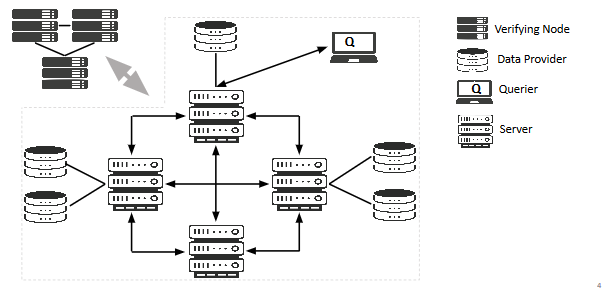
\includegraphics[scale=0.75]{img/lemal.png}
\caption{System model of Lemal}
\end{figure}
Lemal is a privacy-preserving data sharing system, as an enhancement of UnLynx \cite{unlynx}, and this project is part of its development. It consists of a collective authority (CA) formed by $m$ servers, $S_1,...S_m$ and $n$ data providers $DP_1,...DP_n$ containing sensitive data, encrypted using Elliptic Curve (EC) ElGamal.
Another collective authority of verifying nodes (VNs) is linked to this system and maintains a distributed ledger. It is described in Section 5. This system as a whole is used to answer queries made by a querier $Q$, to produce results of some aggregate functions. Each DP chooses one server of the CA to communicate with and can change this at any given time.\\
\textbf{Functionality}: Lemal enables a large set of SQL queries, like \textit{where, group by, like, mean, variance, set intersection}, with some machine learning (\textit{linear and logistic regression}) and private recommender system functionality such as \textit{cosine similarity, CBF-Based recommendations, among others.}.\\
For any query, some zero-knowledge proofs are generated by the CA server. These are used to prove that the servers did the computations correctly, with respect to the privacy of the data, but also with respect to the correctness of the results. They are randomly verified by each node of the VNs and stored in a Skipchain so that any party can verify what is correct. It is also possible to access all the proofs and verify them.\\
\textbf{The pipeline} of the model is as follow:
\begin{itemize}
\item{Data providers send data with/without Range Proofs to the CA servers and verifying nodes}
\item{The CA executes a collective aggregation protocol and sends the proof to the VNs}
\item{The CA executes a verifiable shuffling protocol and sends the proof to the VNs}
\item{The CA executes a key switch protocol and sends the proof to the VNs}
\item{This part is the main goal of the project. Each VN verifies each proof with a given probability, set in the query. When all proofs have been received, a \textit{block}, which is basically a structure containing information of what has been verified and for which query, is inserted inside the Skipchain}
\item{The CA sends to the querier its result(s), and the block is in the ledger (if correct)}
\end{itemize}

\subsection{Threat Model}
In this section, the assumptions made about the parties taking part in the general protocol are detailed.
\begin{figure}[H]
\center
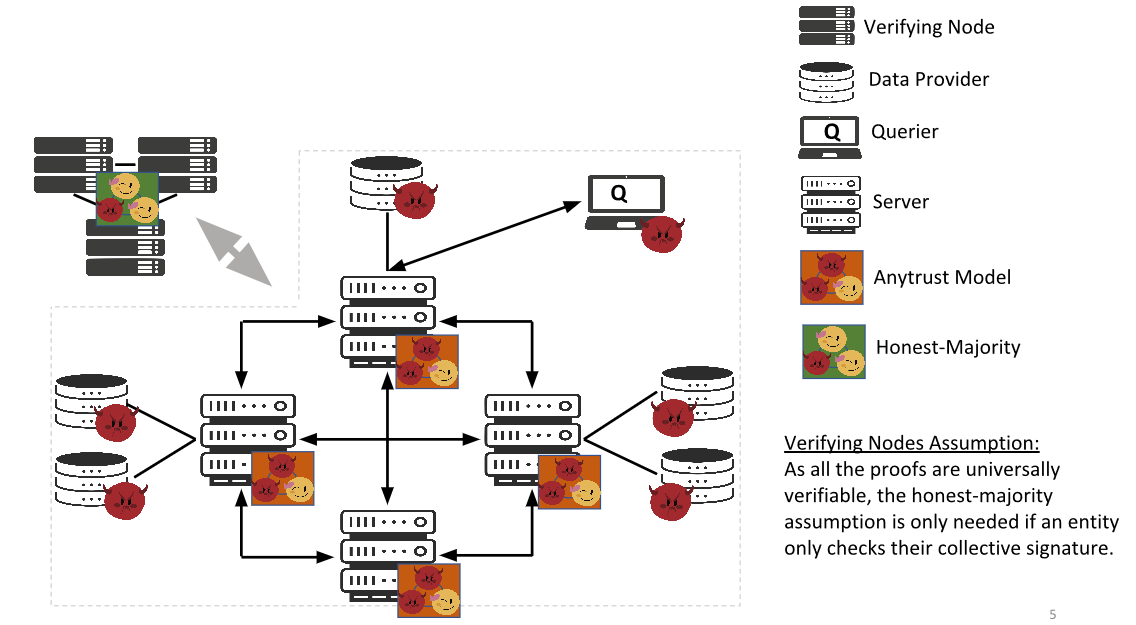
\includegraphics[scale=0.5]{img/threatLemal.png}
\caption{Threat model of Lemal}
\end{figure}
\textbf{Collective authority servers} It is assumed an Anytrust model \cite{anytrust}. It does not require a particular server to be trusted or to be honest-but-curious. Whenever one of the servers is not malicious, correctness, security, and privacy are guaranteed.\\
\textbf{Collective authority verifying nodes} We assume an Honest majority. Meaning a threshold of more than half of the nodes is honest, and the consensus is done via Byzantine Fault Tolerance (BFT) protocol. This way, a consistent timeline is kept for the chain of blocks, and all data inserted on the chain are verified. Indeed, only one node of the VNs will start the insertion of data (root node), that were collected from all the nodes and a consensus will be run to verify these data.
\textbf{The Querier, and Data providers} are assumed malicious. They can collude between themselves or with a subset of the CA servers.\\
It is also assumed that all network communication is encrypted and authenticated by using a protocol such as TLS or SSL.
\subsection{Properties}
In this section, we present the properties guaranteed by the system. The first subsection brings up the already existing properties coming from UnLynx, while the second one introduces the properties guaranteed by the work done in this project.\\

\subsubsection{Properties guaranteed by UnLynx}
\textbf{Confidentiality} All data are encrypted using EC-ElGamal, no party sees the data in clear, except the Querier that gets the aggregate result encrypted under his/her public key. This property holds as long as one server is not malicious.\\
\textbf{Privacy} The system ensures \textbf{differential privacy} for any individual sharing its data.\\
In all cases, the privacy of the querier is not addressed in this system, as we only care for the sensitive data of the DPs.\\
\subsubsection{Properties guaranteed by Lemal}
\textbf{Correctness} At each step of the protocol, zero-knowledge, non-interactive proofs are generated by the CA servers or the DPs. These proofs can be used between two steps of the protocol to verify that computation was correctly done, and if it is not the case, any entity can identify a subset of entities responsible for the wrong computation.\\
This is a property of UnLynx, but is handled by the VNs CA.\\
\textbf{Robustness} is ensured through the distributed ledger. In case of faulty computation, the block contains the verification of proofs at each server, as well as the identity of the issuer of these proofs.
If there is an incoherence in these verifications, the block also contains a way to retrieve all the proofs from the VNs CA.\\
Anyone can verify and identify the server/DP or a set of them that cheated or made the proofs incorrect.\\
This way, these malicious parties can be excluded from the protocol.

\subsection{Query example}
This subsection exemplifies the pipeline of a query process, to highlight the generated proofs and information sent to the developed skipchain service.\\
First, the querier $Q$ sends a query to the CA servers. The example taken in this section is "SELECT average(x) FROM y WHERE y.z $< 321$".\\
This query is received by a server $s$ of the CA and broadcasted to the entire CA. Then each server sends the query to its DPs. The DPs execute the query locally, then send the result encrypted with the CA's public key back to the servers.\\
The first proof is sent to each node of the VNs, proving that the cipher resulting from each DP is in a given range, if a range was specified.\\
At this point, each server of the CA contains ciphers encrypted with the CA's public key.
Then, a collective aggregation is carried out. In the current example, the server will add the ciphers and the root server (the one the querier contacted) will initiate an aggregation protocol, to get the final result, which is in this example, the sum of each server's data and the total number of values summed. This protocol is done using a tree implementation. Children servers will send their aggregated values to their parent, who will aggregate them, and the same thing will happen until the top of the tree is reached.\\
Again, a proof is generated, which is just the ciphers before and after aggregation, and is sent to the VNs.\\
At this point, there might be differential privacy applied to perturb end-result in order to satisfy privacy. In this example, servers might collectively add some noise, that does not make the whole mean varies too much, but that gives privacy on the number of values and individual result for each server.\\
This comes from UnLynx with Distributed Results Obfuscation (DRO) step, that enables the CA to collectively and homomorphically add noise, sampled from a probabilistic distribution.
To do so, a shuffling phase is initiated, where multiple sequences of noise values are randomly permutated. This ensures that the noise is randomly chosen for a given query.\\
This shuffle is also verifiable, a proof is generated at each server when its execution is finished and sent to the VNs.\\
Finally, the servers engage in a key switch protocol. It permits to sequentially add values to the final result to obtain an encryption under the public key of the querier. To do so, each server adds an element containing a nonce and its public key. A  proof of what it has computed is created. Again, the proofs are sent to the VNs.\\
To finish the process, the root server sends back the result to the querier.\\


Note that we did not include the Verifying nodes process in this query example, but only what they receive. In the next section, we further detail the operations performed by the verifying nodes.

\section{Verifying  Node}
This section presents the implementation of the Verifying nodes CA. It was the main goal of this project and will be the major part of this report. We will first present in details the threat model and the theoretical system model, then the supported operations, and in the following section the chosen implementation strategy.\\
\subsection{System Model}
The verifying nodes CA's goal is to reduce the proofs verification time of a querier or any entity wishing to verify the operations for a specific query, by doing the computations, and storing data related to the proofs inside a block of a distributed ledger. This also ensures correctness as proofs verifications are stored in an immutable way, and we provide a way to retrieve proofs to identify faulty parties, i.e. to guarantee robustness.\\
In order to optimize the time overhead of verifying all proofs, several modifications are done.\\

When a query is received by the CA,  the exact number $P$ of each type of proof expected from each entity is known by the verifying nodes. So the CA sends to the VNs the query, and it computes $P$ to initialize a dictionary that will be referred as "\textit{bitmap}" from now on. This bitmap is used to keep track of the proofs received from the CA and that have been processed. It is a way to link each proof to its verification without having them to store all proofs' structure inside the block. So a proof is referenced as a string and its verification as an integer, inside the \textit{bitmap}. Of course, each node of the VNs has its own bitmap.\\

Then, proofs are sent as soon as they are created to all nodes of the VNs CA, as seen in Section 4.4. To be sure that the proofs are coming from the correct entity, all of them are signed by the server/DP that issued it, and the signature is verified before processing it.\\
Each node verifies the proof probabilistically with a fixed threshold $p \in (0,1]$. Thus, each server has a different subset (with high probability) of verified proofs, that might intersect. This redundancy is desirable for verification of proof, as it increases the probability that the proof is indeed correct/incorrect.\\
The verification result i a $1$ if the proof is correct, $0$ if incorrect, $2$ if it has not been verified, and 3 if the proof has not been received (set by a timeout).\\
After verifying these proofs, the node stores the result of the verification in the bitmap with the query ID, identity of verifier and creator, as well as the type of the proof as key and the verification result as the value in a local database. The proofs' structure is also stored in this database.\\

To be more precise, when a proof $p$ is sent by a server $s$ to a node of the VNs $v$, for a query with ID \textit{queryID} it randomly verifies it, and stores $2$ values:\\
\begin{figure}[H]
\center
(1) bitmap[\textit{queryID}+\textit{"typeOfProof"}+identity($s$)+identity($v$)] = verif($p$)\\
(2) (\textit{queryID}+\textit{"typeOfProof"}+identity($s$)+identity($v$),$p$)
\end{figure}
Where \textit{"typeOfProof"} can be in this context: \textit{range, aggregation, shuffle} or \textit{keyswitch}.\\
This bitmap (1) is saved in the local database for each query when all proofs have been processed, and will be stored in the Skipchain. This is done so that the service can access the bitmap stored by itself in another service. The values are deleted as  soon as the block has correctly been inserted.\\
However, each proof (2) is stored with the same key in a local database and can be retrieved using the queryID.\\

The VNs then wait for other proofs of the same query to be received, and do the same for all other types of proofs.\\
Upon receiving the last proof, i.e. when the bitmap has been entirely filled, each server gathers all results of verifications inside a unique bitmap, and a protocol to transfer all bitmaps to the root server is launched.\\
At the end of this protocol, the root node launches an insert (or a create chain if there is none yet) block operation given the bitmap aggregated, the query ID, the probability used to select the proof to verify and a timestamp.\\
A verification function runs on all nodes to verify that the root node has not tried to insert malicious data, but the one collected from all the nodes in the previous protocol.
Here we ensure that the data inserted are coherent between the nodes of the VNs CA, meaning that each node verifies that the data it has sent to the root node is inserted in the block.\\
This is different from the proofs verification system, as this check of data inside a block before it is inserted can contain proofs that are not correct, and would still be inserted. This is to identify the entity from which each proof comes from. It can then be excluded from the system if it is judged as malicious.\\
If the block is correctly formed, and the automatic verification depicted previously passes, then the VNs CA inserts the block, otherwise, it is discarded. The verification done by each server is checking whether its bitmap appears in the data of the new block request. If it does not appear it means the root node tried to falsify information.\\
Any client can fetch the last block of the Skipchain at any time.\\

As a summary, the protocol is presented step by step in chronological order:
\begin{itemize}
\item{The query is received by the CA, the exact number of proofs $P$ is known and set for this query.}
\item{The query is broadcasted to the DPs, that send their data to the CA, and range proofs to the VNs if and only if there is a need for range proof. The proofs are signed by the DPs.}
\item{The CA servers processes the data, creating proofs at each step. They are signed and sent to the VNs.}
\item{Upon receiving a proof, a node verifies the signature, then verifies the proof with probability $p$, if it was expecting more proofs of this type,  and stores the proof in a local DB.}
\item{When all proofs have been processed, each node stores its final bitmap in its database and a protocol to insert a block is launched by the root node.}
\item{The root node gathers all the \textit{bitmaps} and passes them as data to insert a new block, as well as a timestamp and the queryID.}
\item{Inside the block insertion service, each node verifies that the data from the final \textit{bitmap} contains its data, by comparing the received data with the one stored inside the local database.}
\item{If the block was well formed and the previous verification was correct, the service returns the newly added block, containing the bitmap from all servers, timestamp, query ID, and threshold as data.}
\end{itemize}
\subsection{Threat Model}
As described previously, the threat model of the VNs CA is Honest-majority. This means that at least half of the servers are honest. This property must hold in order to maintain the Skipchain correctly. Indeed, an adversary must compromise at least half the servers, to violate correctness and to make the insertion of a forged block possible, without being rejected.

\subsection{Types of Proofs}
As described in section 4.4, the CA servers generates different kinds of proofs. This subsection will present in details what they contain and how they are verified. All these proofs come from UnLynx framework \cite{maxproject,unlynx}.\\
\textbf{Range proofs} are computed by each DP. They prove that a commitment $C$ is in a range $[a,b]$. These are used to handle malicious DP input. In a query with range predicate, they are perfect to prove that an encrypted value indeed lies in a given range, without leaking the value itself. These proofs were designed to compare Prio and UnLynx in a previous project \cite{maxproject}.\\
A modification was done in this project such that each structure of proof contains a list of range proofs, if an entity sends multiple range proofs, it can send them in one request. They are \textbf{optional}, as it is possible that a query does not contain range predicates.\\
\textbf{Shuffle proofs} are computed by the CA servers to prove privacy. They ensure the privacy of previously verified data, with differential privacy via noise addition. They serve the purpose of assessing that the noise added has been randomly chosen.\\
\textbf{Aggregation proofs} are also computed by the CA servers. They ensure correctness of computation, without leaking any information on data, except the information that the operation leaks itself. For example, a MEAN operation will leak the number of data that the CA aggregates. They are used to verify the ciphers before aggregation and the resulting aggregation.\\
\textbf{Key Switch proofs} are computed by the CA servers. These proofs ensure the security of data, and correctness of computations. Their goal is to prove that the protocol to switch encryption key is correct without leaking the data in clear. They prove that data before and after addition of a value by a server, are coherent.\\

\subsection{Supported operations}
Here, the operations supported by the verifying nodes are presented in details.\\
There are two services that we can distinguish. The first one is the service that handles the verification and storage of the proofs.\\
The second service handles the communication with the Skipchain, as well as the functions and data accepted by the Skipchain.\\ 

\subsubsection{Query and Proof handling}
The first service handles the reception of queries and proofs.
Upon receiving the query, it initializes the bitmap and prepares it for a fixed number of proofs.\\
Then each type of proof described previously in section 5.3 can be handled, verified and stored independently, with each one having its own handler. Each proof must be signed by the entity that issued it to be processed correctly. The storage is done locally at each server using a database (DB).

\subsubsection{Skipchain operations}
The second service is the link between the first one and the Skipchain. It permits to insert a block or create one if no chain existed. It is automatically launched when the bitmap has been fully filled. It calls the service implemented by DEDIS to create/maintain a Skipchain. It takes a structure containing all the data that a block contains as parameters, and returns the block if it has been inserted correctly in the chain.\\
The operations to retrieve blocks are also linked to DEDIS' Service but are described in the next subsection.

\subsubsection{Functions for external clients}
Some functions are available for external clients, to retrieve information from the Skipchain or the VNs.\\
It is possible to get the last block of the Skipchain, as well as a specific block, given its ID (hash), its index or the query ID. This way anyone can access the data in the block (the \textit{bitmap}), to check the verification of the proofs. The servers/DPs that issued the proofs and the nodes of the VNs that verified these proofs are known as they are stored in the \textit{bitmap} as key.\\

There is also a way to access all the proofs for the query the block was created for.\\
Each server of the VNs stores the proofs issued at each query, and a client can ask to any node all or a subset of the proofs for a given query ID.\\
As they are stored in the same key/value way as the verifications, it is easy to identify which nodes verified what proofs, and which DP/server issued them.

\section{Implementation}
In this section, the technical implementation of the VNs CA is detailed. All the implementation was done in an UnLynx branch called Lemal \cite{lemal}.\\
We first present the service that handles, verifies and stores the proofs. Then the service that handles the communication with the Skipchain.\\
Finally, the addition made to the Skipchain service of DEDIS \cite{skipchain} is addressed in the last part, as well as the possible calls that external entities can make to the VNs CA.\\

To make the implementation easier, each DP and server are considered as clients by the Verifying nodes. This way, they can send data and requests using API functions.\\

\subsection{Handlers}
This subsection presents the different handlers of the client and service side, for the proofs.\\

We define a client of the service as an \textit{API} structure, that contains its ID as well as the private key it uses to sign the data it sends.\\
On a verifying node, a Service runs and the structure contains several important fields: A concurrent map that stores all information of a query processing, meaning the size, the bitmap and the query itself. When a proof for this query needs to be handled, these structures will be updated in consequence.\\
The threshold to verify a proof is set by the received query. The local database of each VN is defined using BoltDB \cite{bolt}.\\

The client can call several functions to send data to the Service. The first call expected is \textit{SendQuery}, that broadcasts the query to all the nodes of the VNs CA.\\
These nodes handle the query with the \textit{ReceiveQuery} function, that sets the bitmap size with the number of proofs expected for this query, given its ID, and stores these pieces of information in a concurrent map.\\

Then all the different types of proofs have their own handler.\\
We will describe precisely how one handler works, and generalize for all of them.\\

A range proof is sent by the client using \textit{SendRange}. This function broadcasts to all nodes of the VNs the proof, as well as the signature, the identity of the client and a potential \textbf{SkipBlock}.
The Service receives this proof with the \textit{HandleRange} function, that verifies first if more proofs of this type where expected thanks to the concurrent map, verifies the signature, and verifies probabilistically the proof. Then, it updates the bitmap, and the number of proof expected, and store them back inside the concurrent map. It also stores in its local database the proof.\\
If it is the last proof for this query, after being handled, the insertion process is launched through a function called \textit{checkForInsertion}. This function appends a new block containing all the previously handled proofs for this query, to the \textbf{SkipBlock} given in argument. If it is not the last proof or there is no skipchain yet, this field can be \textit{nil}.\\
This \textit{checkForInsertion} is the return value of each handler. It returns 2 values a skipblock and an error. The first one is \textit{nil} if no insertion has been done, or a \textit{SkipBlock} if it has been correctly done. The second one is an error, it is \textit{nil} if no error occured.\\


To extend about how the proofs verification and proof itself are stored, we explain here how we defined the structure to do so efficiently.\\
The verification of proofs is stored inside a map of (string, integer), as long as the whole query has not been processed. When the block is inserted, it is deleted, as it is stored inside the ledger, and can thus be retrieved. The \textbf{key} of this map is a string of the form : \textit{queryID+"typeOfProof"+clientID+deterministicInfo+nodeID}. The deterministic information is used if the sender of the proof needs to send several proofs of the same type, while keeping the uniqueness of the key. The value is 0,1,2 or 3 in function of the returning value of the verification.\\
For the storage of the proof in boltDB, the same system of key/value is used. The only difference is that the database is split into buckets, that have a maximal capacity. So upon receiving a proof, a bucket is created/loaded with key \textit{queryID+"typeOfProof"}, and the proof is stored with the same key as the bitmap, and the value is the proof in bytes.\\

The same implementation is used throught all handlers. \textit{SendAggregation} and \textit{HandleAggregation}, \textit{SendShuffle} and \textit{HandleShuffle}, \textit{SendKeySwitch} and \textit{HandleKeySwitch}.

\subsection{Skipchain Operations}
There are 2 types of operations on the Skipchain. Inserting a block, or getting one that is already in the chain.\\
The first one is done via the handler, the insertion will begin inside the \textit{checkForInsertion} function when all proofs have been received. If no block was passed as argument a new chain is created, else it is appended at the end of the chain. This is done by calling the \textit{skipchain} Service implemented by DEDIS. It handles all the technical features of the chain itself, and is not the aim of this project and will not be discussed in details.\\
In addition to these functions, anyone can ask for the last block known by the VNs CA given an already known block. The client can call \textit{GetLatestBlock} giving the roster (the set of verifying nodes represented as a structure) that handles the skipchain, and a SkipBlock. The service receives the request with \textit{GetLatestBlockRequest} and sends back the last block it knows.

\subsection{Addition to the Skipchain Service}
A modification has been done to the \textit{skipchain} Service implemented by DEDIS to fit the scenario described in the report. The Service from DEDIS provides a way to register a  verification function that runs on all nodes when a block is received to verify if its structure and data are correct.\\
This is done by adding a registration for this function in our Service. The function is called \textit{verifySkipBlock} and does the following on each node:
\begin{itemize}
\item{It loads the local database, as the service runs on the same node that the one that handled the proof.}
\item{It gets the bitmap saved before launching the insertion}
\item{It verifies that all data from the loaded bitmap are also in the bitmap of the block data request}
\end{itemize}

This way all nodes verify that their data is present in the block and that no malicious party tried to falsify information.\\
As Byzantine Fault Tolerance is used, only a strict majority of nodes needs to suceed the verification to insert the block.\\

\subsection{API for external Clients}
The following functions are useful for parties that are external to the Lemal framework.\\
First, anyone can get all the proofs for a given query. A client can call \textit{GetProofsFrom} with an ID and the node from which it wants to retrieve the proofs. The node returns the map of string to proof in bytes that was stored in its local DB.\\
This map's values can then be transformed from bytes to proof structures (the key contains which type of proof it is) by doing the conversion itself, or by calling \textit{TranformToAllProofs} that will return a structure called \textbf{DataToVerify} containing 4 arrays of proofs, 1 of each type.\\

Of course, one might also want to retrieve a block for a given query. The \textit{GetBlockForQuery} return the block that corresponds to the given queryID.\\

Eventually, if a client has no block, it can ask for the genesis one that is stored in the local database of all nodes. This way it can retrieve the last block and explore the chain. The client call \textit{GetGenesis}, give a verifying node identity, that will fetch in its DB the block and returns it.

\section{Performance Evaluation}
This section presents the performances of the VNs CA with different parameters. All simulations were done on the iccluster of EPFL, with 5 servers \cite{cluster}, using Mininet. For each of our servers, we used machines with two Intel Xeon E5-2680 v3 CPUs with a 2.5GHz frequency, 256GB RAM that supports 24 threads on 12 cores.\\
We evaluate the computation time in function of the number of servers, the number of DPs and the number of VNs. In addition, a graph presenting the verifications times in function of the threshold set in the query is shown at the end.\\
A request is defined as a server/DP sending one of its proof to all the VNs.\\
The simulations are done with 2 queries. All requests (proofs coming from an entity) are sequential, but the sendings to each VN inside a request are parallelized. This means that each node verifies a proof in parallel.\\
As each of the nodes runs the verifications in parallel, the measurements taken are the maximum of the computation time of all the VNs, i.e. the bottleneck.\\


Note that the test data generated use the following specifications for the inputs:\\
Aggregation does the aggregation of $1,2,3,4,5$ encrypted with EC-Elgamal, with 2 grouping attributes.\\
The shuffle uses 2 arrays of ciphertexts containing respectively the following value encrypted $1,2,3,6,$ and $2,4,8,6$. \\
The key switch is made on 2 random ciphers.\\
Range proof is made using the range $[0,16^{16}]$, 5 servers and the value $25$ encrypted.
\subsection{Scaling in number of Data Providers}
We first present Figure 3, that shows the verification time of Range proofs for a varying number of DPs (from 1 to 200) and fixed parameters.
\begin{figure}[H]
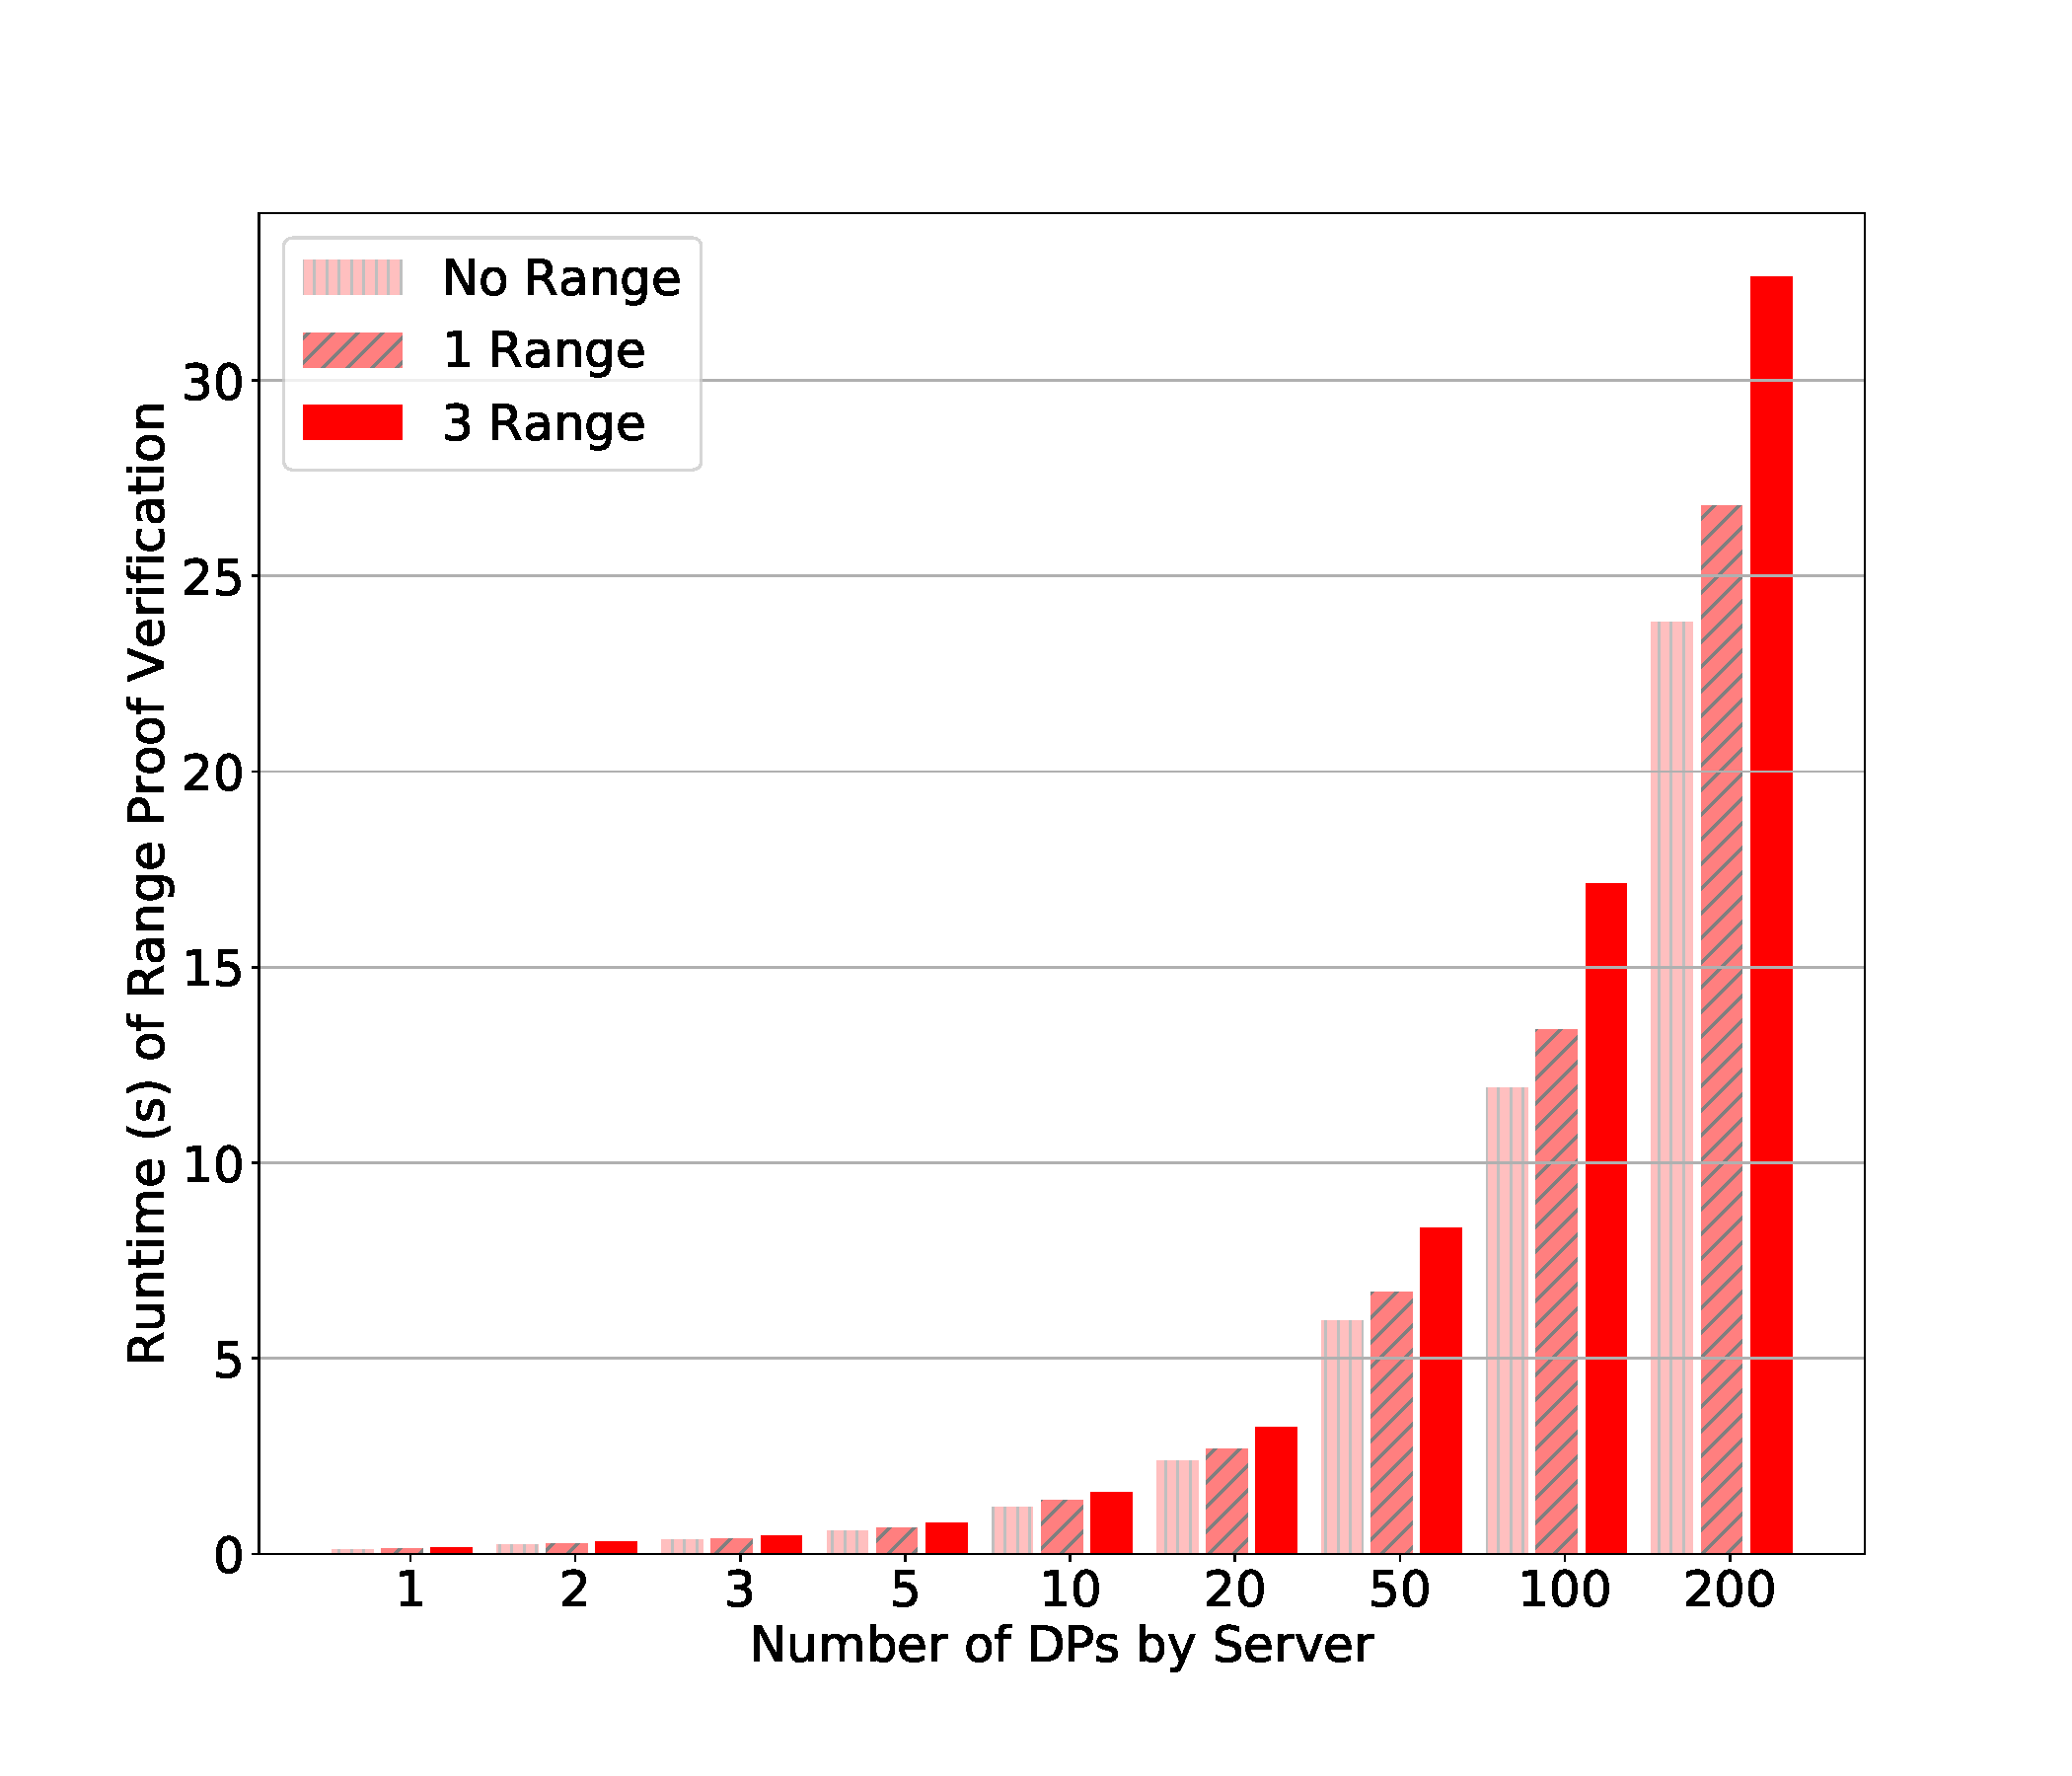
\includegraphics[scale=0.5]{variationInDPRange}
\caption{Variation of the number of DPs by Server, for 5 Servers, 5 Verifying Nodes and Threshold = 1.0}
\end{figure}
This graph only presents the variation of range proofs verification, as all the other proofs verifications are constant (they vary with the number of servers). 3 bars are shown, one with a proof containing no range predicate, a second one with 1 range in the request, and the last one with 3 range predicates inside the request. This is still one proof as the structure contains a rangeList.\\
Note that 100 DPs by server means that each  DP sends its proofs to each VN. In this context, we have 5 servers meaning $100*5 = 500$ range proofs to verify.\\
First, all verifications grow linearly, with a value of 17 seconds for 3 ranges at 100 DPS and around 33 seconds for 200 DPs.\\
The difference between the bars (number of range proofs by request) for a same number of DPs is the interesting difference to explain. There is a small difference between the no range and 1 range with 12 seconds versus 13 seconds for 100 DPs by server. This is due to 3 main reasons. First, the verification phase contains a signature verification, that takes the same time for every structure, even with no range proofs. This signature verification is done even if the proof is not verified probabilistically by the VN due to the threshold value.\\
The second reason is that the proofs verification is efficiently parallelized, explaining the low difference between 1 range and 3 range proofs, i.e. it does not grow by a factor of 3 (13 seconds for 1 range proof and 17 seconds for 3 range proofs at 100 DPs by server).\\
Moreover, in the simulations done, the range proofs verification were always not correct due to some compatibility problems. This is still a good approximation of the execution time, as every sending will later be perfectly parallelized in addition of the parallel verifications.

\subsection{Scaling in number of Servers}
Figure 4 presents the verification time of proofs for a varying number of Servers (from 3 to 50) and fixed parameters.

\begin{figure}[H]
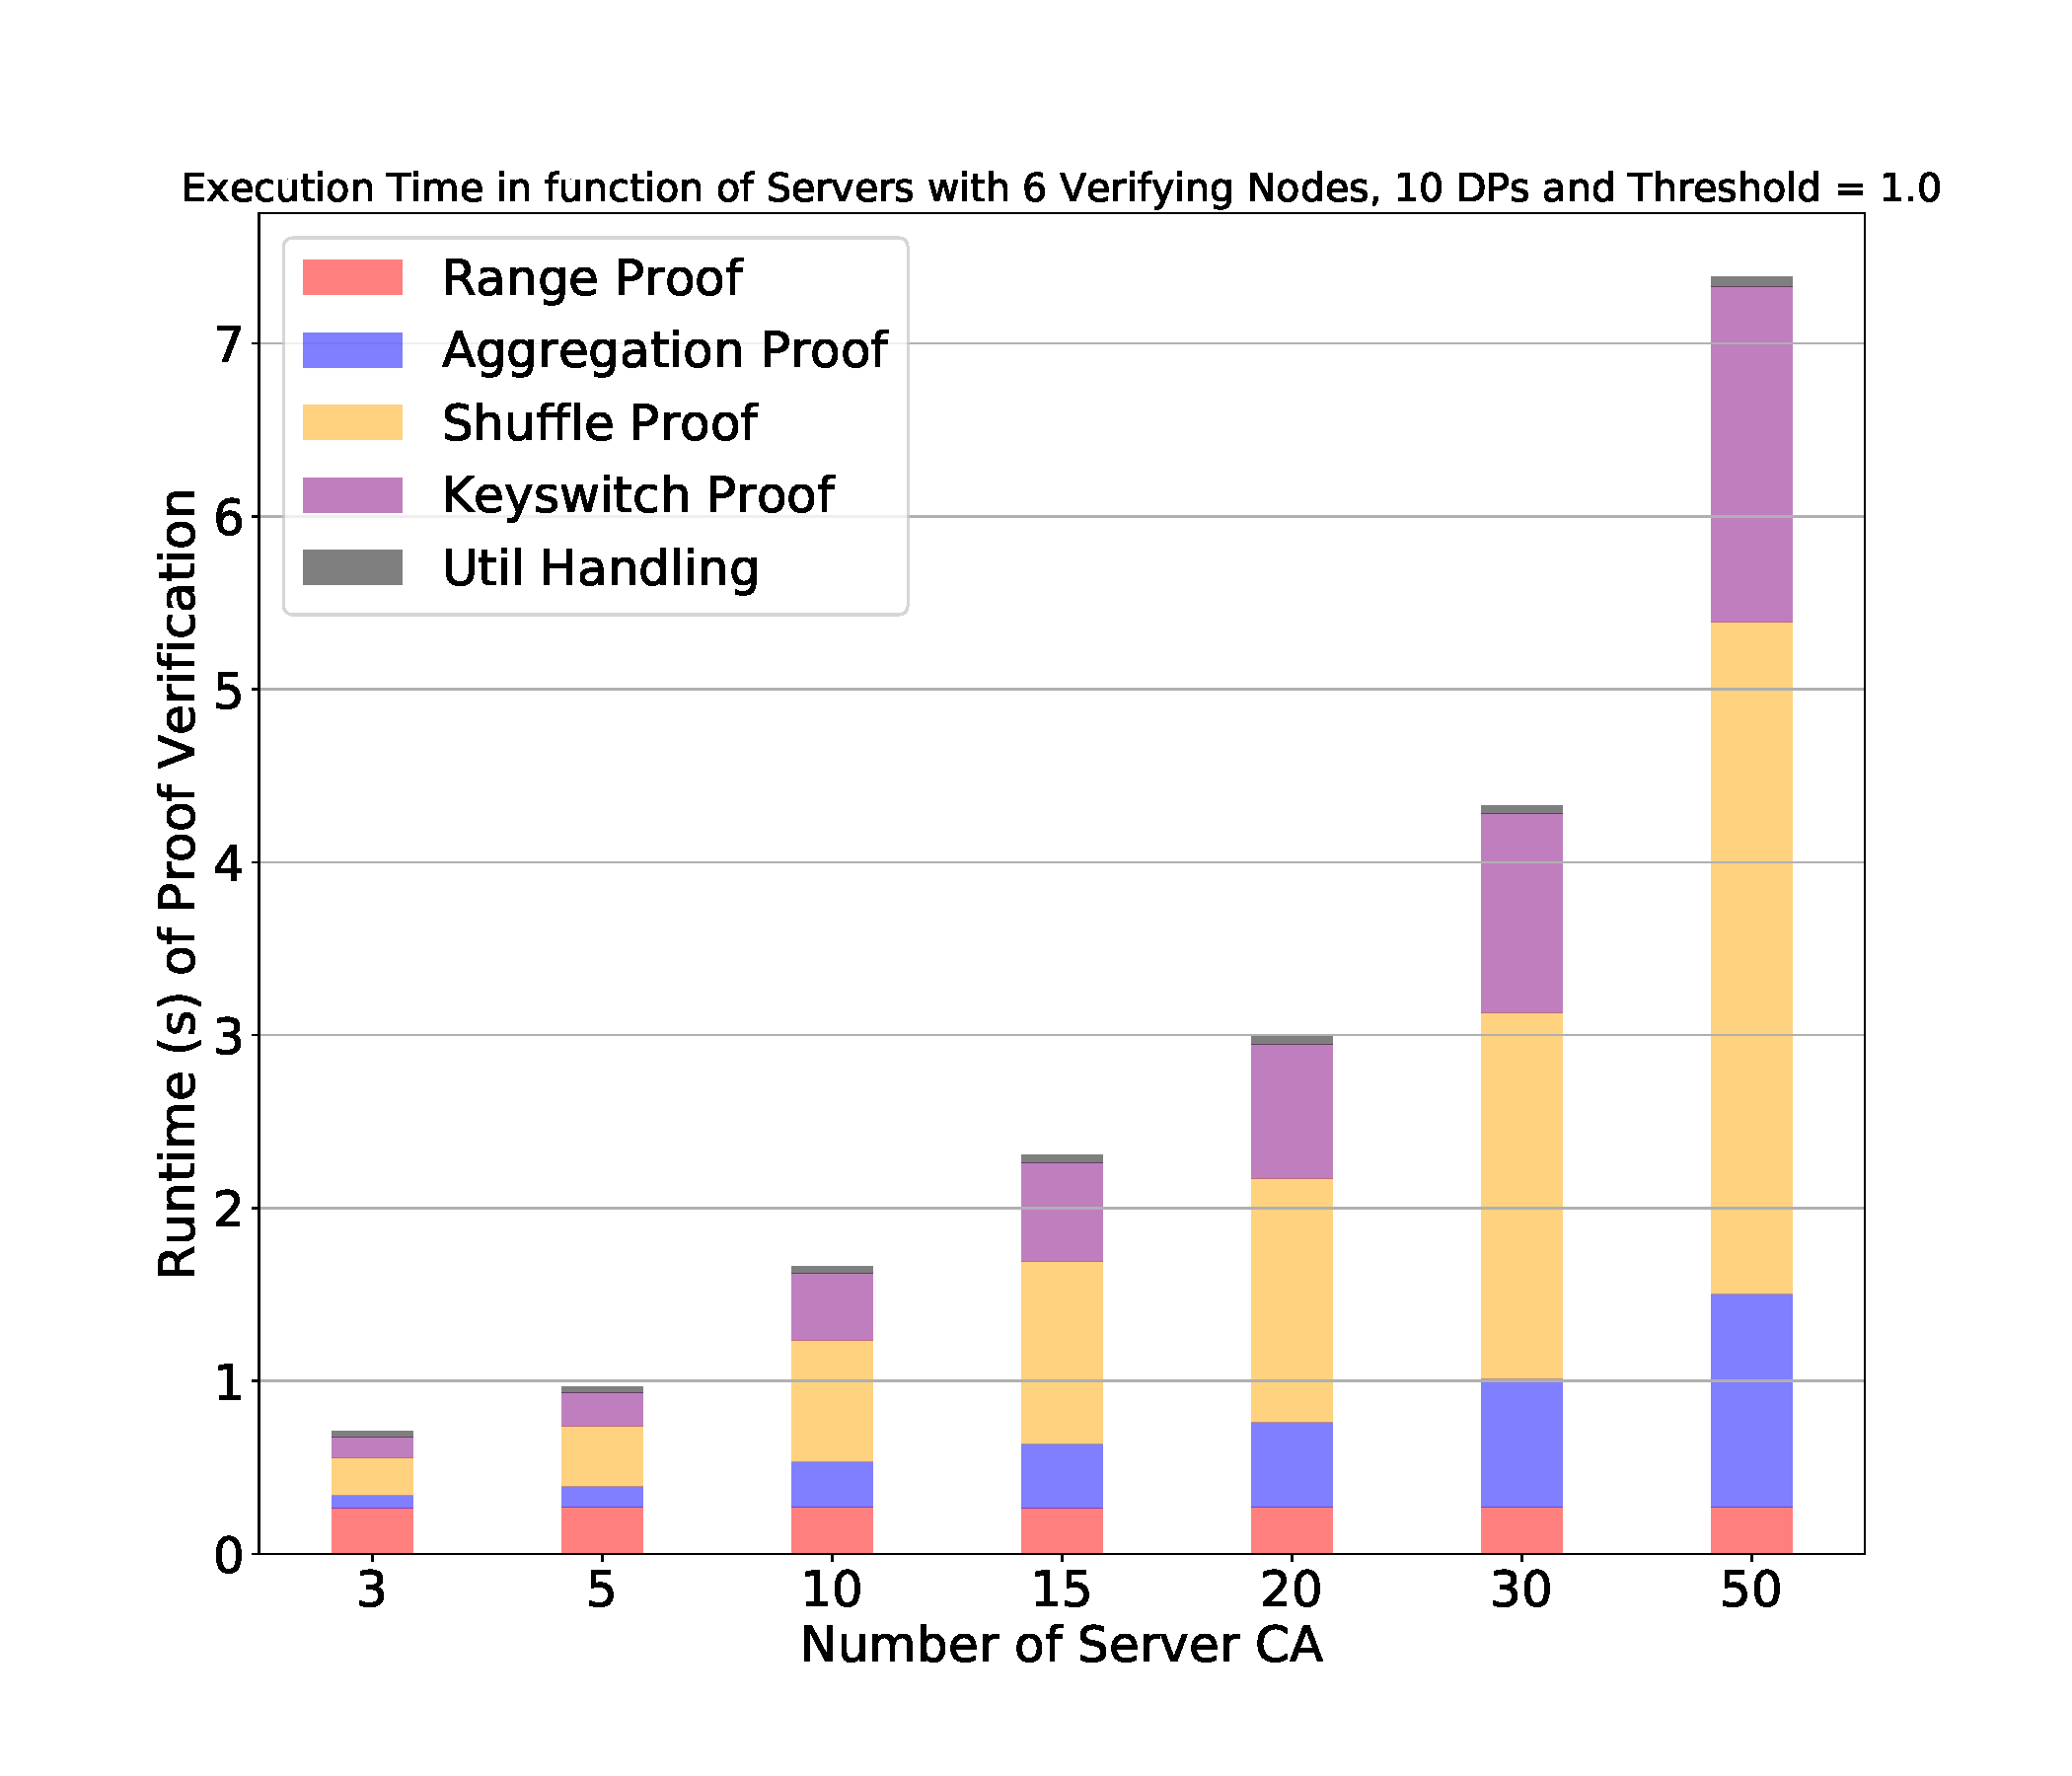
\includegraphics[scale=0.5]{variationInServ}
\caption{Variation with the number of Servers}
\end{figure}

Here we present the variation of proofs verifications, the range proofs are shown but will not be addressed as they are constant with the number of DPs that is fixed to 10 here (10 total and not 10 by server).\\
So 10 servers means that there are 10 verifications of shuffle, keyswitch and aggregation proofs.\\
The \textbf{Util handling} is the sum of the time to insert a genesis block, then insert another block, but also the time to collect the bitmap for both these blocks and the time to return a block after asking for the last block of the chain.\\
This corresponds to the creation of a skipchain (genesis block) by a first query, then the insertion of a second block (second query), the time that the VNs take to gather the data before inserting both blocks, and finally the time it takes to return the last block of the skipchain when asked. All these times are gathered as they are really small compared to the proofs verifications, i.e. it is around 0.1 seconds.\\
The lowest verification time is the aggregation proof. It grows linearly with the number of servers.\\
It is the same for shuffle and key switch proofs, that grows linearly with the number of servers. From 2 seconds to 4 seconds for 30 and 50 servers for the shuffle, and 1 second to 2 seconds for 30 and 50 servers for the key switch.\\
The Util Handling time also grows but is really low compared to the verifications. Thus, the operations linked to the Skipchain are not a bottleneck for the system, when the number of server increases.

\subsection{Scaling in number of Verifying Nodes}
Figure 4 deals with the operations linked to the skipchain for a varying number of VNs (from 3 to 20) and fixed parameters.

\begin{figure}[H]
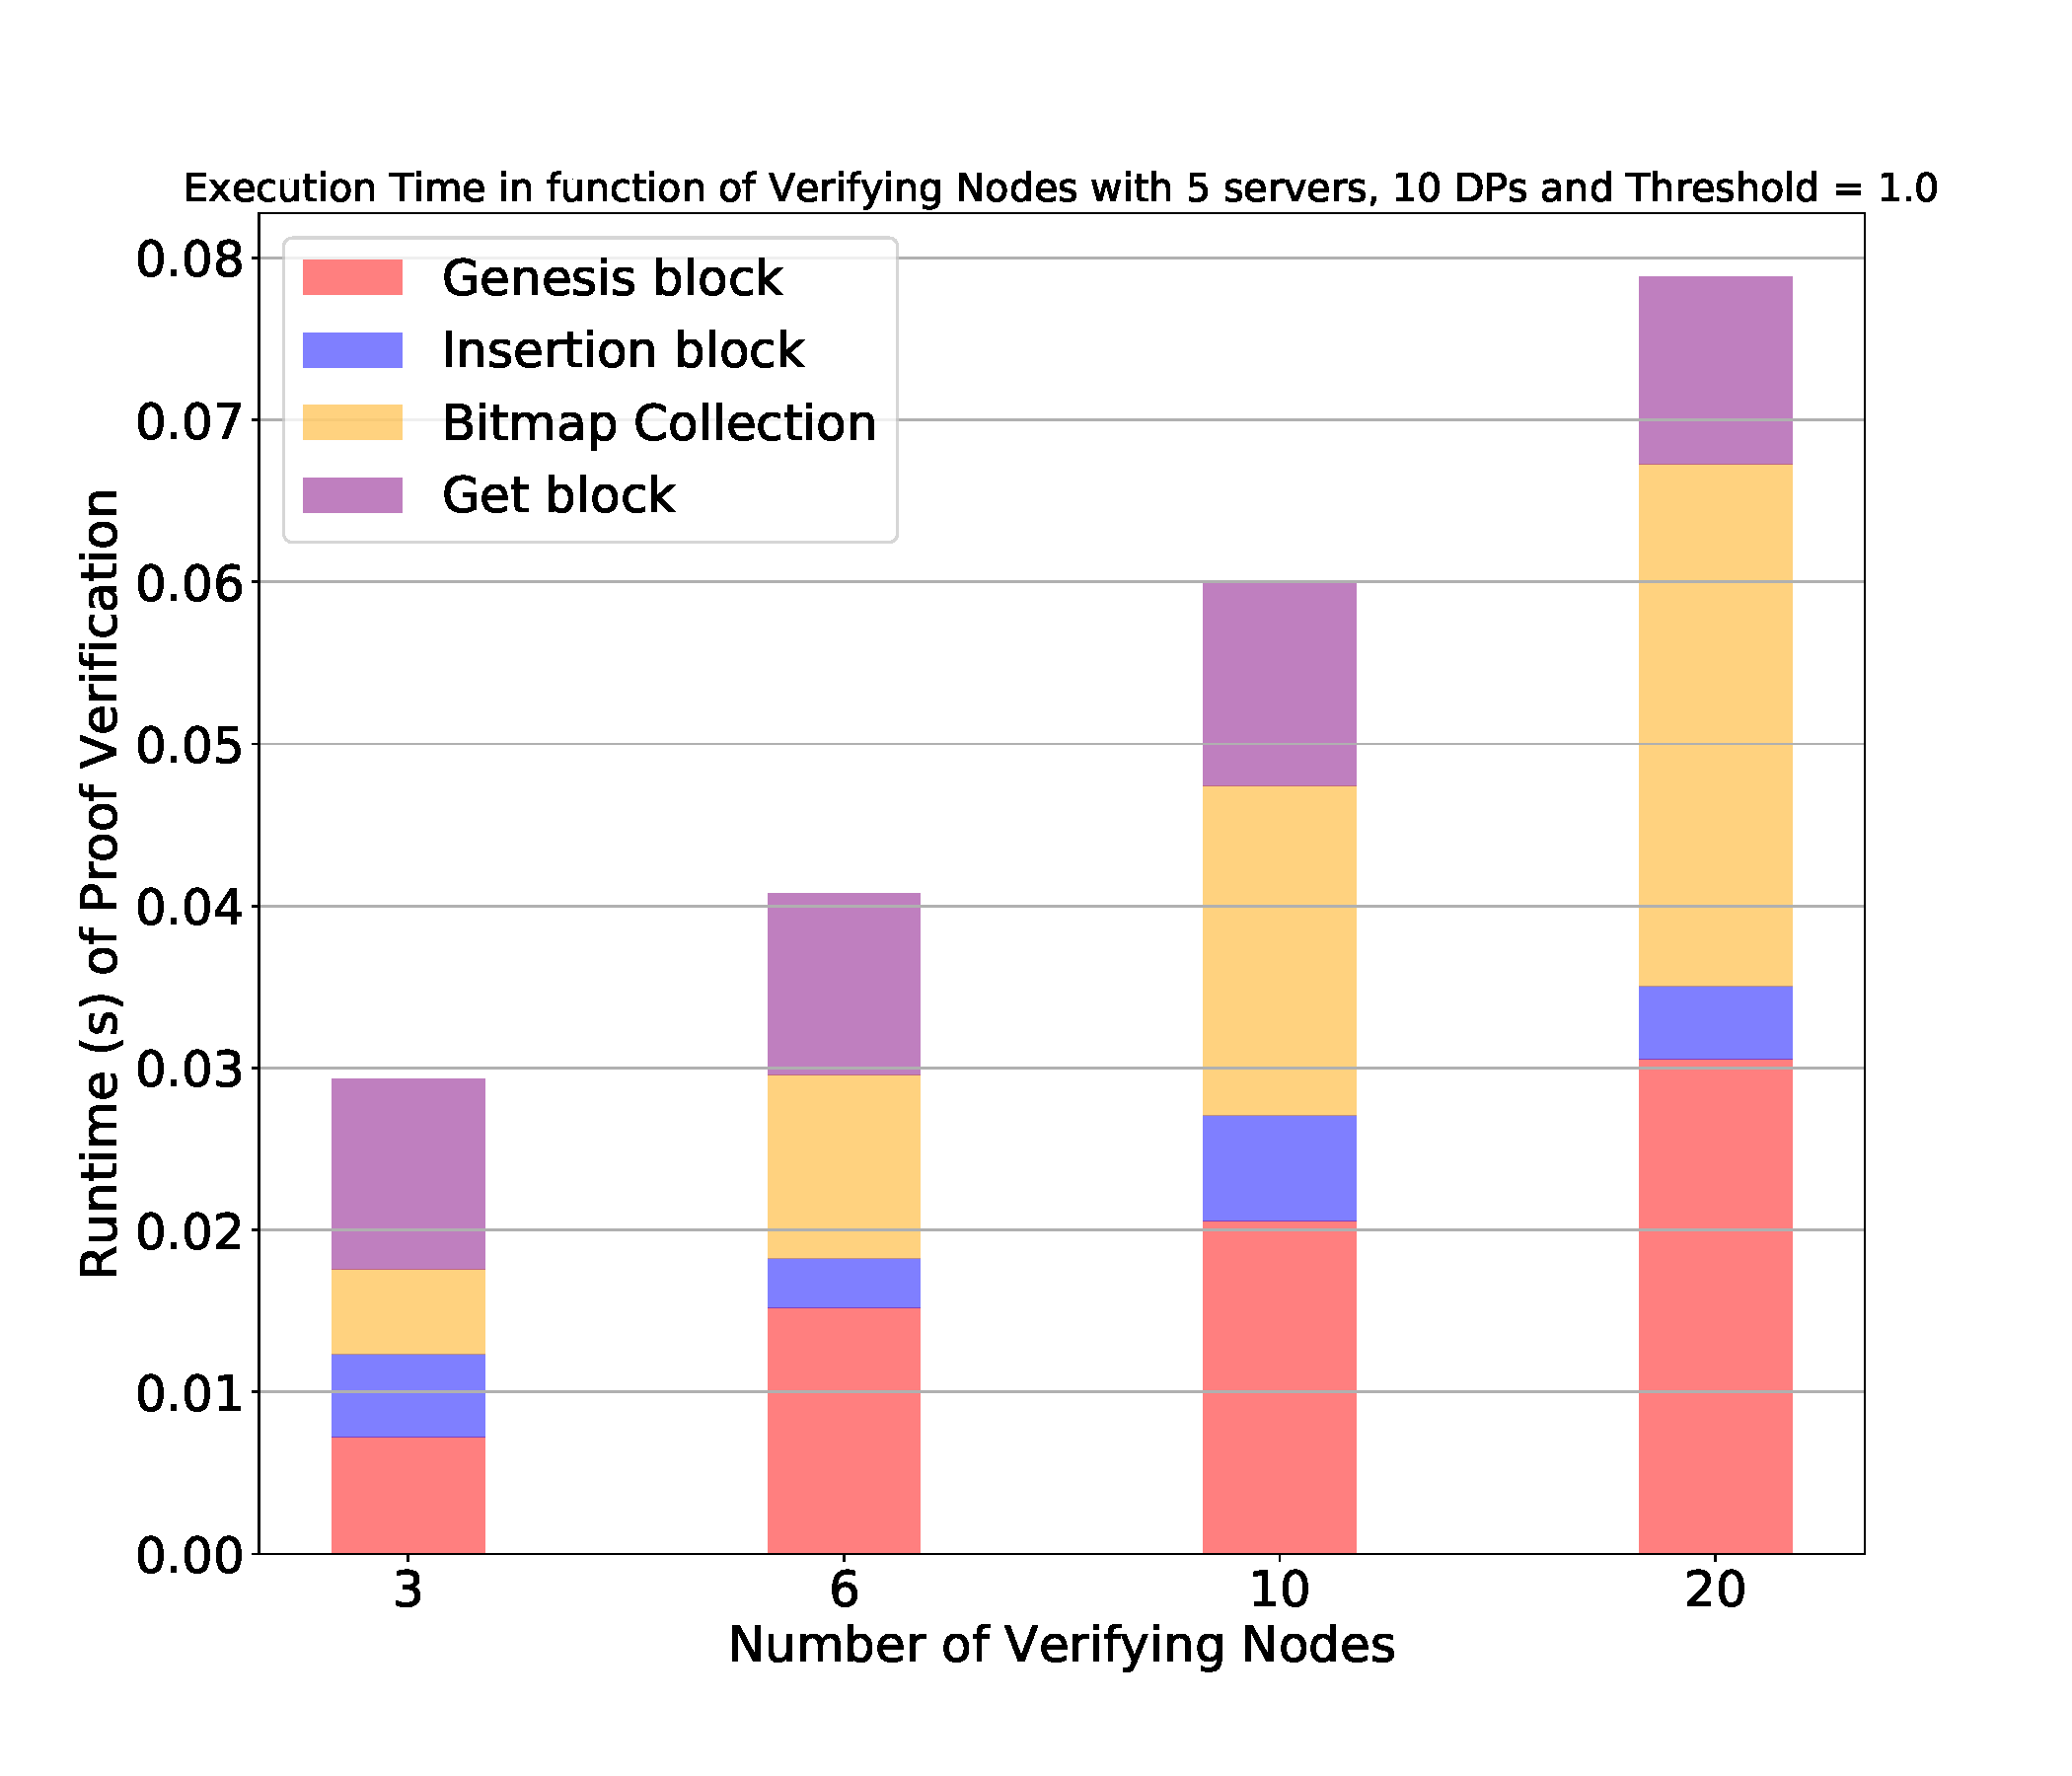
\includegraphics[scale=0.5]{variationVN}
\caption{Variation with the number of Verifying Nodes}
\end{figure}


This graph shows the variation of Skipchain's operations with the number of VNs. The proofs verification time stays constant, as the number of servers is fixed to 5 and the number of DPs to 10.\\
First, we can notice that the time to insert the genesis block is growing linearly with the number of VNs. It goes from $0.005$ second for $3$ VNs to $0.015$ for $6$ of them.\\
The time to insert a block does not seem to follow a linear growth, as the insertion might depend on the propagation and verification of the block on each node.\\
The time to get a block is almost constant as if there are less than $10$ nodes, the node receiving the request will ask all the nodes and will return the block with low latency time (around $0.1$ second). The propagation of messages is optimized and of a really small order (around $0.01$ second). If there are more than $10$ nodes, the node receiving the request will ask half the nodes. The value for getting a block is $0.0112$ second for $6$ nodes, and $0.0125$ second for $10$ nodes.\\
Eventually, the time to collect the bitmaps from all the nodes grows linearly with the number of VNs, which makes sense as the more VNs there are, the more bitmaps and data the root needs to collect.

\subsection{Threshold variation}
The last variation is depicted in Figure 6. It shows the proofs verifications time with the threshold variation. The number of servers is fixed to 10, the VNs to 6, and the number of DPs to 10.\\

\begin{figure}[H]
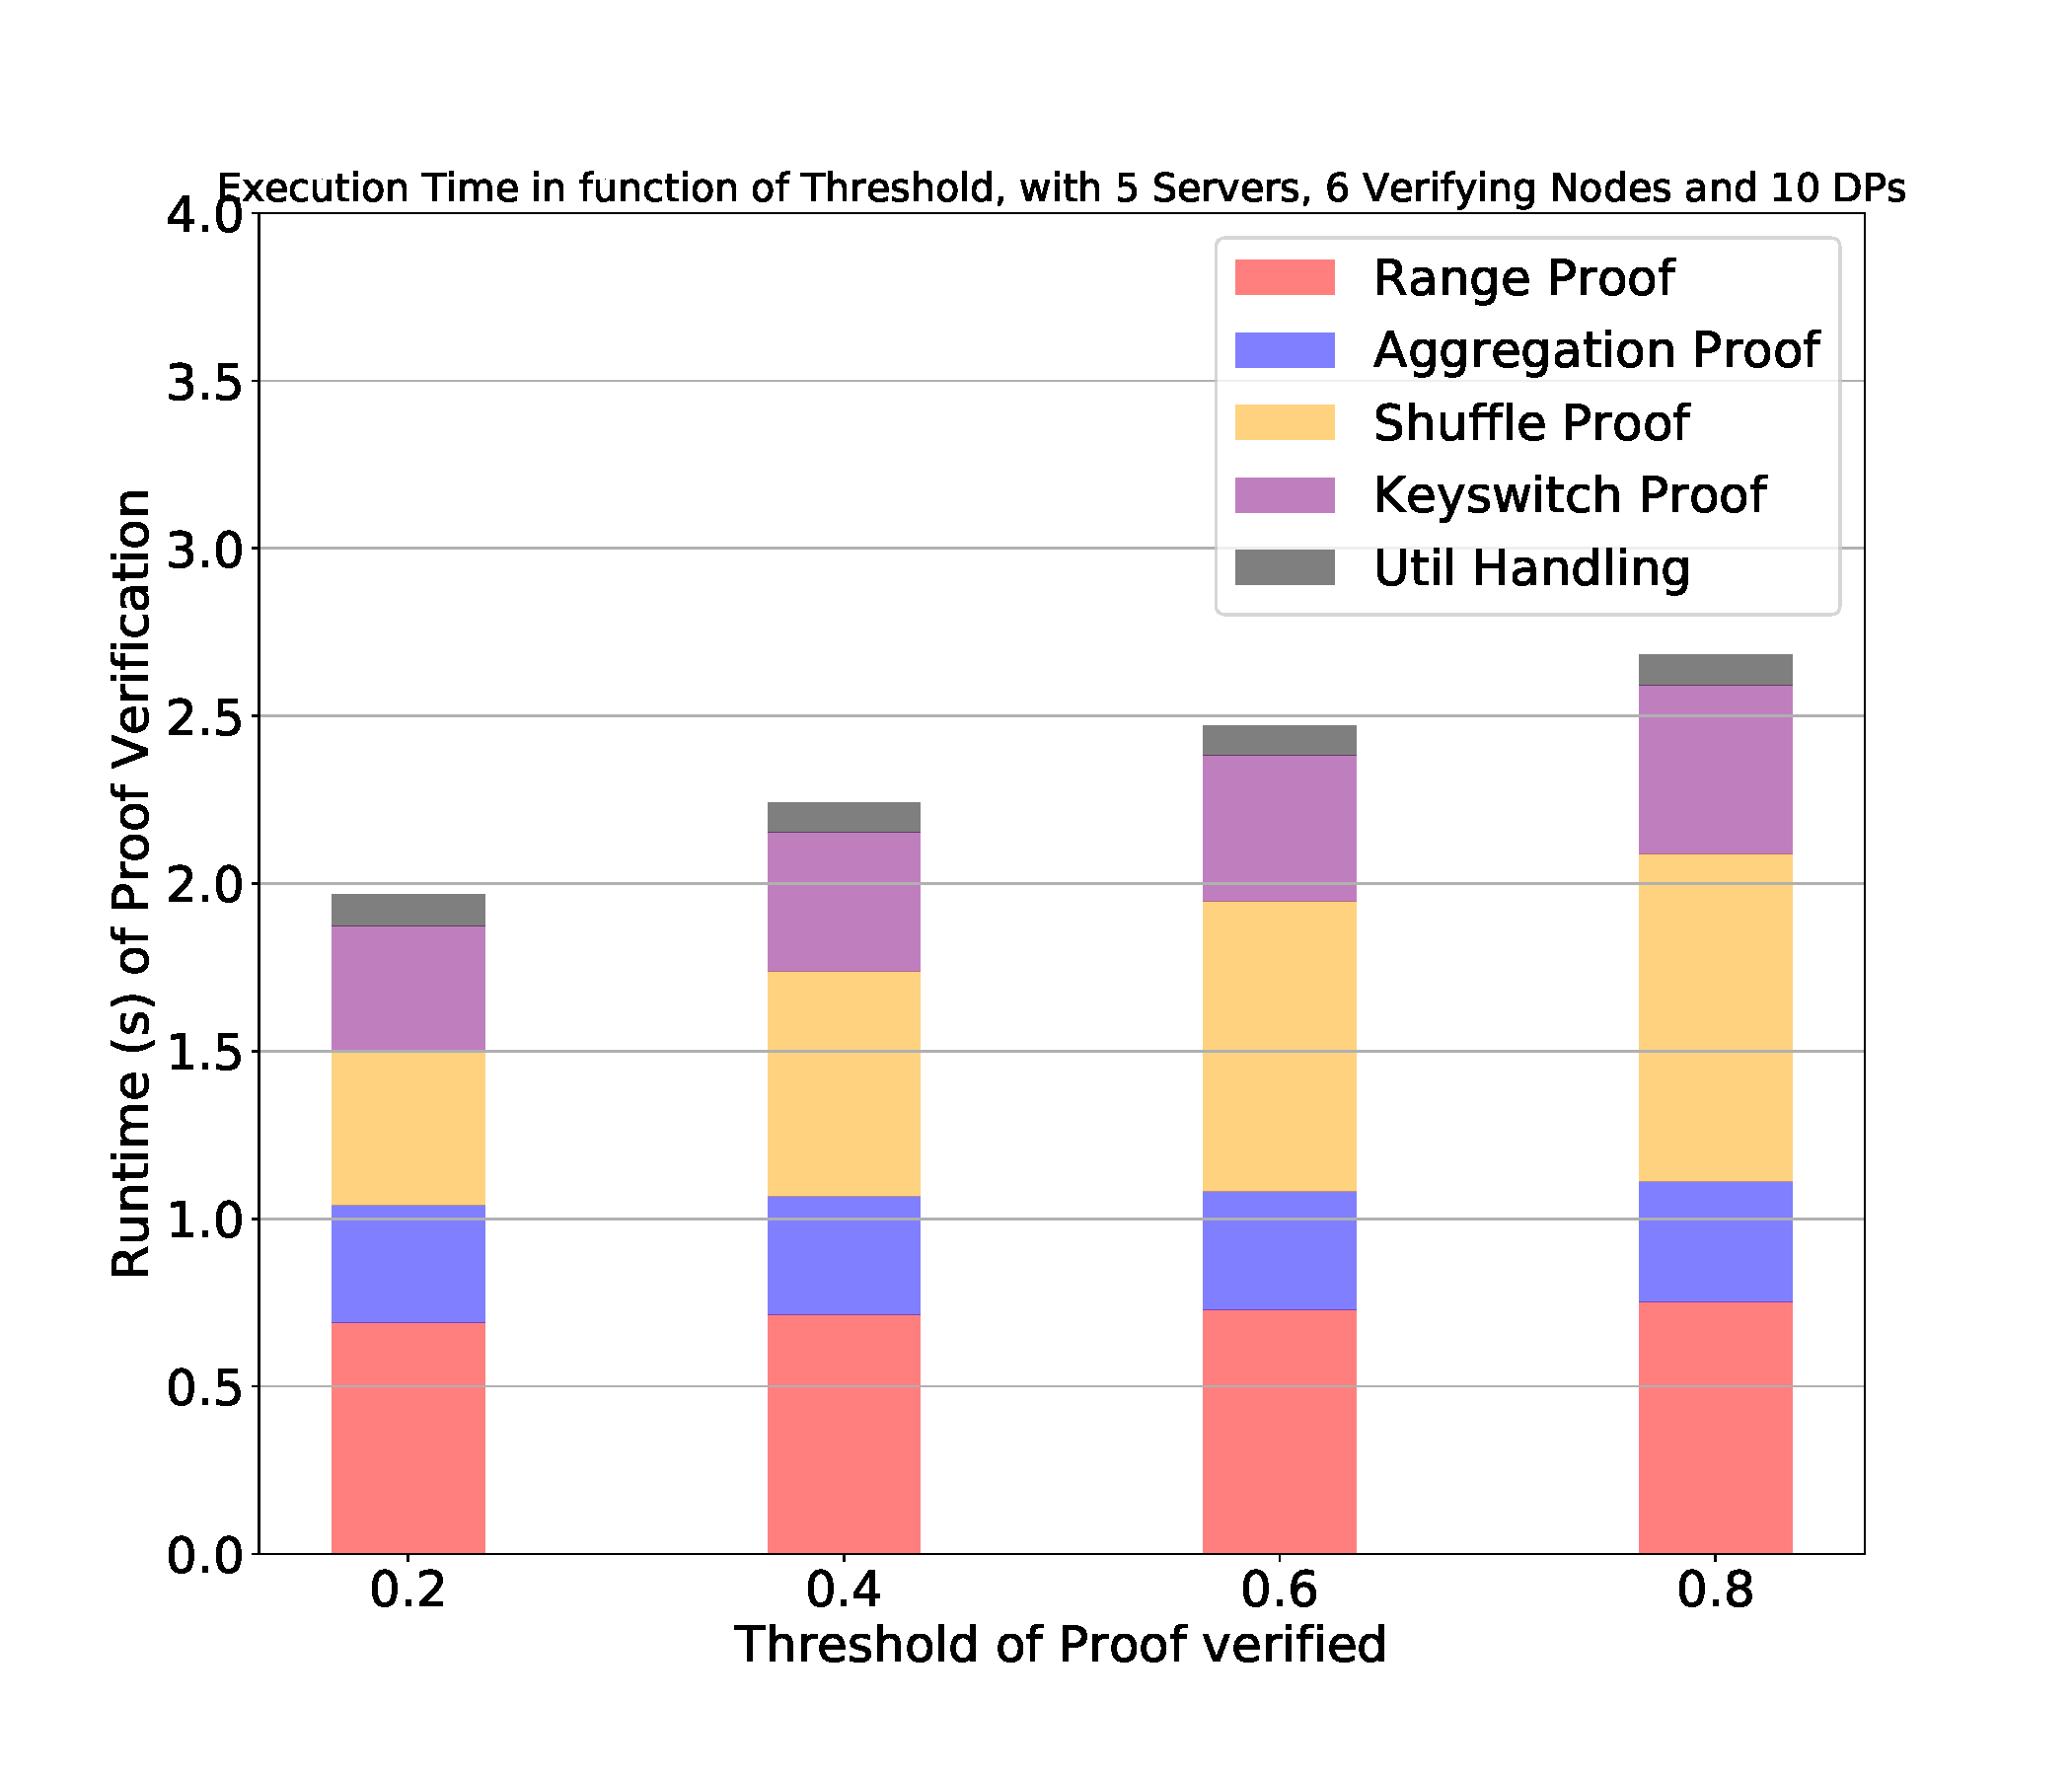
\includegraphics[scale=0.5]{variationWithThreshold}
\caption{Variation in function of the query Threshold}
\end{figure}

First, the execution time of Range proofs has a really small growth (0.704 second for 0.2 and 0.752 second for 0.8). This is mostly due to the fact that the proofs fail almost immediately when they are verified, and the difference between a verification and none is of order 0.01 second. It is the same for the aggregation with even smaller value (0.346 for 0.2 and 0.357 for 0.8). This is due to the fact that aggregation verification is really efficient and quick. The differences are not visible or too small to be noticed.\\
However, for shuffle and key switch, the execution time grows linearly with the threshold.\\
The Util Handling is constant for varying threshold, which makes sense as it does not affect any skipchain operation.\\
Note that the verifications times are really low, and even if they are not verified, proofs' signature is still checked.

\subsection{Bandwidth}
This section presents the size of the proofs and requests sent from DPs/Servers to VNs.\\


Each request contains the same fields. An ID referencing the query, the senderID referencing which entity sent the proof, and a potential deterministic information, which is used to keep the key unique for different proofs from one same entity. Each of these fields are \textit{string} type.\\
Then the signature and the data of the proof are both arrays of bytes. The signatures are of constant size, but the data of proofs will vary in function of which type of proof is handled.\\
Finally, a roster and a skipblock are also in each request, even if the block is often \textit{nil}.\\
The roster is used in each request to specify the VNs CA that will handle the request. It also permits to avoid sending the request to a subset of servers, as it verifies if the block previously inserted had the same roster than the current one.\\
The skipblock needs to be specified if and only if a request is the last one for a given query, and that the block created should be appended to the block given. If it is not the last one, the VNs will fetch it from the given one.\\


Table 1 presents the sizes of the proofs structures as well as the size of the entire request containing the previously stated elements. The signature is always 96 bytes, and strings are really small, and a mean size of 20 bytes is taken for them.\\

\begin{table}[H]
\centering
\caption{Size of proof for the simulations ran}
\label{my-label}
\begin{tabular}{|
>{\columncolor[HTML]{656565}}c |c|c|}
\hline
{\color[HTML]{FFFFFF} Type of Proof} & \cellcolor[HTML]{656565}{\color[HTML]{FFFFFF} Size of Proof} & \cellcolor[HTML]{656565}{\color[HTML]{FFFFFF} Size of Request} \\ \hline
{\color[HTML]{FFFFFF} Range}         & 45568 bytes                                                  & 45976 bytes                                                    \\ \hline
{\color[HTML]{FFFFFF} Shuffling}     & 8518 bytes                                                   & 8926 bytes                                                     \\ \hline
{\color[HTML]{FFFFFF} Aggregation}   & 3934 bytes                                                   & 4386 bytes                                                     \\ \hline
{\color[HTML]{FFFFFF} Key Switch}    & 1331 bytes                                                   & 1739 bytes                                                     \\ \hline
\end{tabular}
\end{table}

We can see that the bottleneck is clearly the range proof which is a lot bigger (by a factor of 5 for shuffling, 11 for aggregation an 40 for key switch) than all the other proofs. This is due to pairing points that are of size $384$ bytes, while a classic point of EC-ElGamal is $64$ bytes.

\section{Conclusion and Future Work}
This project achieves an implementation of a Distributed Ledger for Lemal system, based on the Skipchain framework. The threat model is stronger than previous systems such as Prio or UnLynx and has more operations available. Moreover, as the proofs verifications are done in parallel of the CA servers computations, the system achieves a better running time than the framework it was based on, UnLynx.\\

Providing both \textbf{correctness} of results and \textbf{robustness} of computation, the Distributed Ledger allow universal proofs verifications, as well as an entity that computes the proofs verifications instead of the CA servers. Moreover, it introduces a threshold of verification, permitting the VNs CA to compute only a part of the proof, trading correctness for computation time. This trade-off does not make the correctness obsolete, as each VN will verify a different subset of proofs, and there is a high probability that all the proofs are verified and that the verified sets intersect on several verifying nodes.\\

However, some improvements could be made to the system to achieve better performances. We state some guidelines to implement some optimizations that could be done to improve the system further.\\

One of them would be the parallelization of the requests sending by different servers/DPs, that should improve the system computation time.\\
For the bandwidth, modifications could be made to the proofs' structure and verifications. Indeed, there is a redundancy of information that could be removed. For example, the output of a keyswitch proof of a server is the input for the next server's key switch proof. Such modifications could also be applied to shuffle proofs.\\
Then, we saw that the range proof is also a really big part of the bandwidth, we could look for another pairing that may be smaller in term of size.

The system is still in development and needs some changes to make everything works perfectly as theoretically planned. An example would be the range proofs that always fail due to versioning of some cryptographic libraries.\\

Eventually, such a system as a whole should be subjected to a security analysis, as well as performance to be sure that it outperforms previously developed data sharing systems.

\newpage
\begin{thebibliography}{9}
\bibitem{prioimple}
Henry Corrigan-Gibbs, Prio prototype implementation\\
\texttt{https://github.com/henrycg/prio}
s
\bibitem{chainiac}
Kirill Nikitin, Eleftherios Kokoris-Kogias, Philipp Jovanovic, Linus Gasser, Nicolas Gailly, \textit{CHAINAC: Proactive Software-Update Transparency via Collectively Signed Skipchains and Verified Builds}\\
\texttt{https://www.usenix.org/system/files/conference/usenixsecurity17/sec17-nikitin.pdf}

\bibitem{anytrust}
David Wolinsky, Henry Corrigan-Gibbs, Bryan Ford and Aarong Jonhson, \textit{Scalable anonymous group communication in the anytrust model. In 5th European Workshop on System Security. 2012}

\bibitem{bitcoin}
Satoshi Nakamoto, \textit{Bitcoin: A Peer-to-Peer Electronic Cash System}\\
\texttt{https://bitcoin.org/bitcoin.pdf}

\bibitem{lemal}
\textit{Lemal repository}
\texttt{https://github.com/lca1/unlynx/tree/lemal}

\bibitem{unlynx}
David Froelicher, Patricia Egger, Joao Sa\' Sousa, Jean Louis Raisaro, Zhicong Huang, Christian Mouchet, Bryan Ford and Jean-Pierre Hubaux, \textit{UnLynx: A Decentralized System for Privacy-Conscious Data Sharing}\\
\texttt{https://petsymposium.org/2017/papers/issue4/paper54-2017-4-source.pdf}

\bibitem{dedis}
\textit{Decentralized and Distributed Systems}\\
\texttt{https://dedis.epfl.ch/}

\bibitem{health}
Heather Fraser, \textit{How Blockchains can provide new benefits for Healthcare}\\
\texttt{https://www.ibm.com/blogs/think/2017/02/blockchain-healthcare/}

\bibitem{spending}
\textit{Double-spending problem}\\
\texttt{https://en.wikipedia.org/wiki/Double-spending}

\bibitem{coinmarket}
\textit{Diverse Information about Crpyptocurrencies}\\
\texttt{https://coinmarketcap.com/}

\bibitem{skipchain}
\textit{Skipchain implementation repository}\\
\texttt{https://github.com/dedis/cothority/tree/master/skipchain}

\bibitem{maxproject}
Max Premi, David Froelicher, Juan Troncoso-Pastoriza, \textit{Decentalized Data Sharing System based on Secure Multi-Party Computation}

\bibitem{bft}
\textit{Byzantine-Fault Tolerance}\\
\texttt{https://en.wikipedia.org/wiki/Byzantine\_fault\_tolerance}

\bibitem{skiplist}
William Pugh. \textit{Skip Lists: A probabilistic Alternative to Balanced Trees.}\\
\texttt{http://courses.cs.vt.edu/cs2604/fall05/wmcquain/Notes/Supplemental/PughSkiplistPaper.pdf}


\bibitem{bolt}
\textit{Bolt DB documentation}
\texttt{https://github.com/boltdb/bolt}

\bibitem{cluster}
\textit{ICcluster specifications}\\
\texttt{https://install.iccluster.epfl.ch/Portal/}

\end{thebibliography}
\end{document}
